\documentclass[11pt]{article}

\usepackage[left=1in, right=1in, top=1in, bottom=1in, paperwidth=8.5in, paperheight=69in]{geometry} 

\usepackage{graphics,epsfig,graphicx,float,subfigure,color}
\usepackage{algorithm,algorithmic}
\usepackage{amsmath,amssymb,amsbsy,amsfonts,amsthm}
\usepackage[small,bf,up]{caption}


\usepackage{soul}
\usepackage{comment}
\usepackage{url}
\usepackage{boxedminipage}
\usepackage[sf,bf,small]{titlesec}
\usepackage[textsize=footnotesize]{todonotes}
\usepackage[plainpages=false, colorlinks=true,
   citecolor=blue, filecolor=blue, linkcolor=blue,
   urlcolor=blue]{hyperref}

\usepackage{amsmath}

\include{ogmacros}

\newcommand{\bdm}{\begin{displaymath}}
\newcommand{\edm}{\end{displaymath}}

\newcommand{\ben}{\begin{enumerate}}
\newcommand{\een}{\end{enumerate}}

\newcommand{\p}{\partial}
\newcommand{\bs}{\boldsymbol}

\usepackage{amssymb}

\parskip 1ex

\parindent 0ex

\begin{document}
\pagestyle{empty}

\begin{center}
{\large {\bf MATH 140: Mathematical Methods for Optimization}}\\
{\bf Assignment 4---Spring 2024}\\
{\bf Due February 13, 2024} \\
{\textcolor{red}{\bf By:Ronald Nap}}

\end{center}

\textcolor{red}{
Note: Hessian's and Derivatives computed using Wolfram Alpha
}

\begin{enumerate}

  \item ({\bf 10 points}) Consider the unconstrained optimization problem
  \bdm
  \min f(x,y) \equiv - \cos x \cos (y/10).
  \edm
\ben
\item Find and classify all stationary points in the region 
  $-\pi/2 \leq x \leq \pi/2, -10\pi/2 \leq y \leq 10\pi/2$

\begin{enumerate}
    \item[\textcolor{red}{Solution:}] 
    \textcolor{red}{
The function given is $f(x, y) = -\cos(x) \cos(y/10)$. To find the stationary points, we first compute the gradient of $f(x, y)$:
}

\textcolor{red}{
\[
\nabla f(x, y) = \left( \frac{\partial f}{\partial x}, \frac{\partial f}{\partial y} \right).
\]
}

\textcolor{red}{
The partial derivatives are:
}

\textcolor{red}{
\[
\frac{\partial f}{\partial x} = \sin(x) \cos\left(\frac{y}{10}\right),
\]
}

\textcolor{red}{
\[
\frac{\partial f}{\partial y} = \frac{1}{10} \cos(x) \sin\left(\frac{y}{10}\right).
\]
}

    \textcolor{red}{
    To find the stationary points, we set each component of the gradient to zero within the region \( -\frac{\pi}{2} \leq x \leq \frac{\pi}{2}, -\frac{10\pi}{2} \leq y \leq \frac{10\pi}{2} \). 
    }

\textcolor{red}{
\[
\sin(x) \cos\left(\frac{y}{10}\right) = 0,
\]
}

\textcolor{red}{
\[
\frac{1}{10} \cos(x) \sin\left(\frac{y}{10}\right) = 0.
\]
}

\textcolor{red}{
This results in the only solution being \( x = 0 \) and \( y = 0 \), as all other potential solutions do not satisfy both conditions simultaneously within the region.} \\


\textcolor{red}{
To classify the stationary point, we examine the second derivatives and the Hessian matrix:
}

\textcolor{red}{
\[
H(f) = \begin{bmatrix}
\frac{\partial^2 f}{\partial x^2} & \frac{\partial^2 f}{\partial x \partial y} \\
\frac{\partial^2 f}{\partial y \partial x} & \frac{\partial^2 f}{\partial y^2}
\end{bmatrix} = \begin{bmatrix}
\cos(x) \cos\left(\frac{y}{10}\right) & -\frac{1}{10} \sin(x) \sin\left(\frac{y}{10}\right) \\
-\frac{1}{10} \sin(x) \sin\left(\frac{y}{10}\right) & \frac{1}{100} \cos(x) \cos\left(\frac{y}{10}\right)
\end{bmatrix}.
\]
}


\textcolor{red}{
At the point $(0,0)$, the Hessian matrix simplifies to:
}

\textcolor{red}{
\[
H(f)_{(0,0)} = \begin{bmatrix}
1 & 0 \\
0 & \frac{1}{100}
\end{bmatrix}.
\]
}

\textcolor{red}{
The determinant of this Hessian matrix is positive, as $\det(H(f)_{(0,0)}) = 1 \times \frac{1}{100} - 0 = \frac{1}{100}$. Since both diagonal elements (which are also the eigenvalues in this case) are positive, it indicates that the stationary point at $(0,0)$ is a local minimum.
}
\end{enumerate}


  
\item There is a portion of the problem region
  within which the Hessian matrix of $f(x,y)$ is positive definite.
  Give expressions for this portion. You should be able to do this
  analytically but I recommend using Matlab/python.


\begin{enumerate}
    \item[\textcolor{red}{Solution:}] 
\textcolor{red}{

\textcolor{red}{
Using 1a), the Hessian matrix $H(f)$ is
}

\textcolor{red}{
\[
H(f) = \begin{bmatrix}
\cos(x) \cos\left(\frac{y}{10}\right) & -\frac{1}{10} \sin(x) \sin\left(\frac{y}{10}\right) \\
-\frac{1}{10} \sin(x) \sin\left(\frac{y}{10}\right) & \frac{1}{100} \cos(x) \cos\left(\frac{y}{10}\right)
\end{bmatrix}.
\]
}

\textcolor{red}{
The determinant of $H(f)$ is:
}

\textcolor{red}{
\[
\det(H(f)) = 0.005\cos(2x) + 0.005\cos\left(\frac{y}{5}\right).
\]
}

\textcolor{red}{
For the Hessian matrix to be positive definite, the determinant must be greater than zero.
}

\textcolor{red}{
\[
 0.005\cos(2x) + 0.005\cos\left(\frac{y}{5}\right) > 0.
\]
}

\textcolor{red}{
This condition is met within the domain where $\cos(x)$ and $\cos\left(\frac{y}{10}\right)$ are both positive or both negative. Given the specified domain $-\pi/2 \leq x \leq \pi/2, -10\pi/2 \leq y \leq 10\pi/2$, $\cos(x)$ is positive for $-\pi/2 < x < \pi/2$, and similarly, $\cos\left(\frac{y}{10}\right)$ is positive for $-10\pi/2 < y < 10\pi/2$. Therefore, within the given domain, the Hessian matrix can be positive definite where $\cos(x)$ and $\cos\left(\frac{y}{10}\right)$ maintain their positive values and satisfy the determinant condition.
}


\end{enumerate}




  
\item Derive expressions for the search directions associated with the
  steepest descent method.


\begin{enumerate}
    \item[\textcolor{red}{Solution:}] 
    \textcolor{red}{
    The steepest descent method moves from the current point in the direction of the most rapid decrease of the function. This direction is opposite to the gradient of the function at the current point. For $f(x, y)$, the gradient is
    \[
    \nabla f(x, y) = \left( \frac{\partial f}{\partial x}, \frac{\partial f}{\partial y} \right).
    \]
    The search direction at any point $(x_k, y_k)$ is therefore
    \[
    d_k = -\nabla f(x_k, y_k) = -\left( \frac{\partial f}{\partial x}(x_k, y_k), \frac{\partial f}{\partial y}(x_k, y_k) \right).
    \]
    For the function $f(x, y) = -\cos(x) \cos(y/10)$, the partial derivatives are
    \[
    \frac{\partial f}{\partial x} = \sin(x) \cos\left(\frac{y}{10}\right),
    \]
    \[
    \frac{\partial f}{\partial y} = -\frac{1}{10} \cos(x) \sin\left(\frac{y}{10}\right).
    \]
    Hence, the search direction for steepest descent at $(x_k, y_k)$ is
    \[
    d_k = -\left( \sin(x_k) \cos\left(\frac{y_k}{10}\right), -\frac{1}{10} \cos(x_k) \sin\left(\frac{y_k}{10}\right) \right).
    \]
    This expression will be used to update the current point to the next point in steepest descent.
    }
\end{enumerate}



  
\item Write a program that performs the steepest descent iterations,
  without a line search, with an exact line search and with Armijo and
  backtracking (as discussed in class).  Note that you will not be
  able to find the value of the optimal step length analytically;
  instead, determine it numerically. {\em Suggestion:} use a built-in
  one-dimensional minimization function such as {\tt FindMinimum} or
  {\tt FindRoot} in {\sc Mathematica} or {\tt fzero} in {\sc Matlab}.



\begin{enumerate}
\item[\textcolor{red}{Solution:}]
\textcolor{red}{
Refer to HW4.py for full code
}

\begin{figure}[H]
\centering
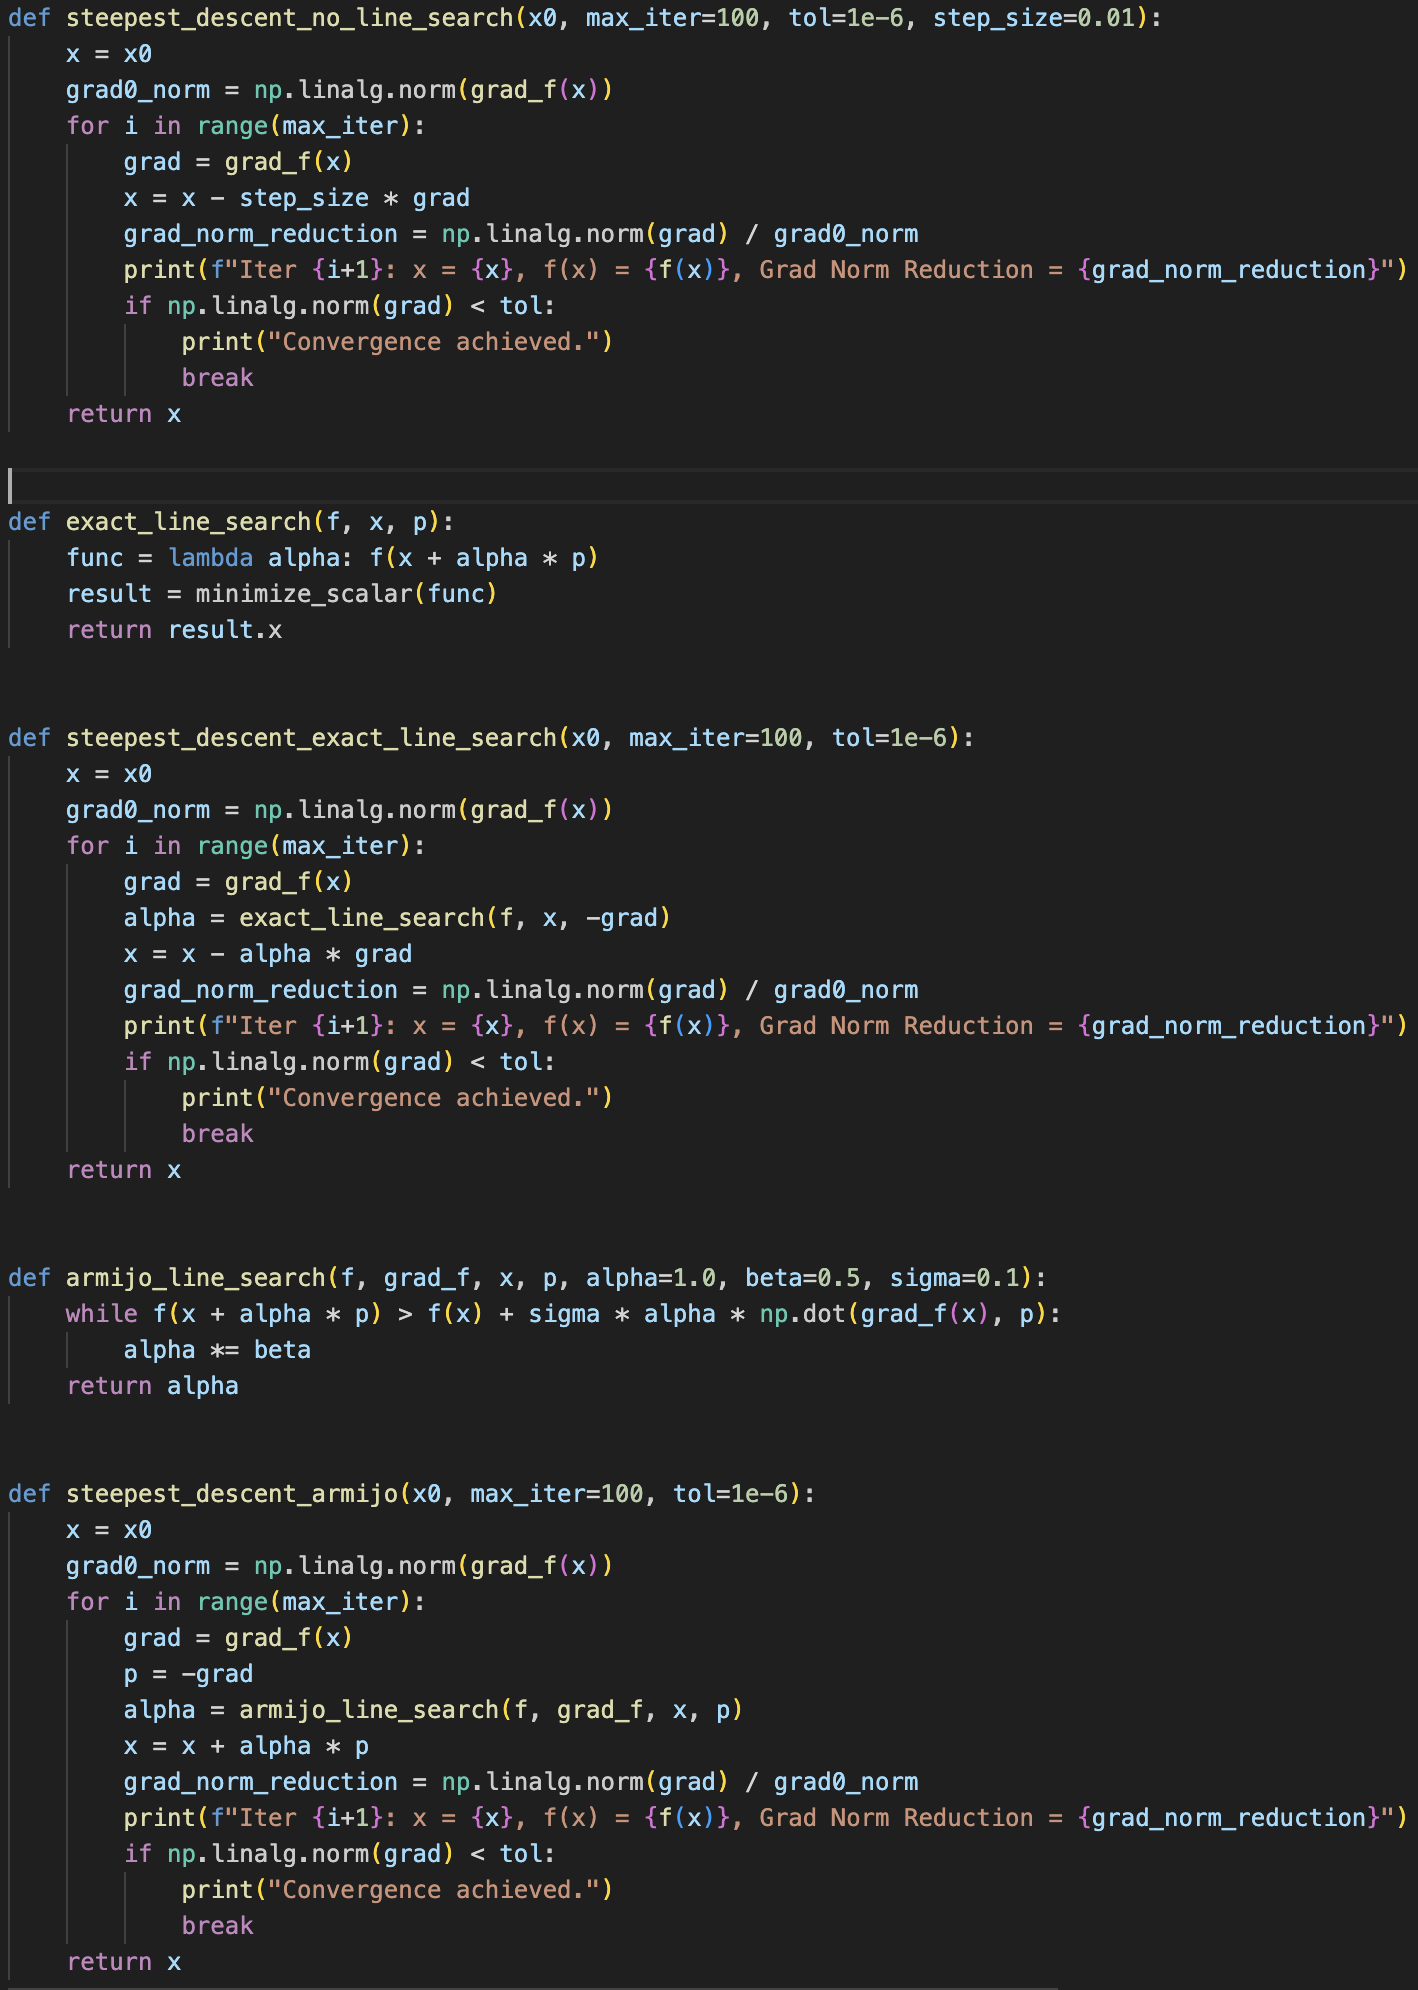
\includegraphics[width=\textwidth]{1code.png} 
\end{figure}

\end{enumerate}






  
\item Run your program for various initial guesses within the region.
  At every iteration print out the
  iteration, the current point $x_k$, the value of the objective
  function $f(x_k)$, and the reduction in the norm of the gradient $ \|\nabla
  f(x_k)\|_2/ \|\nabla
  f(x_0)\|_2$.

    \begin{figure}[H]
    \centering
    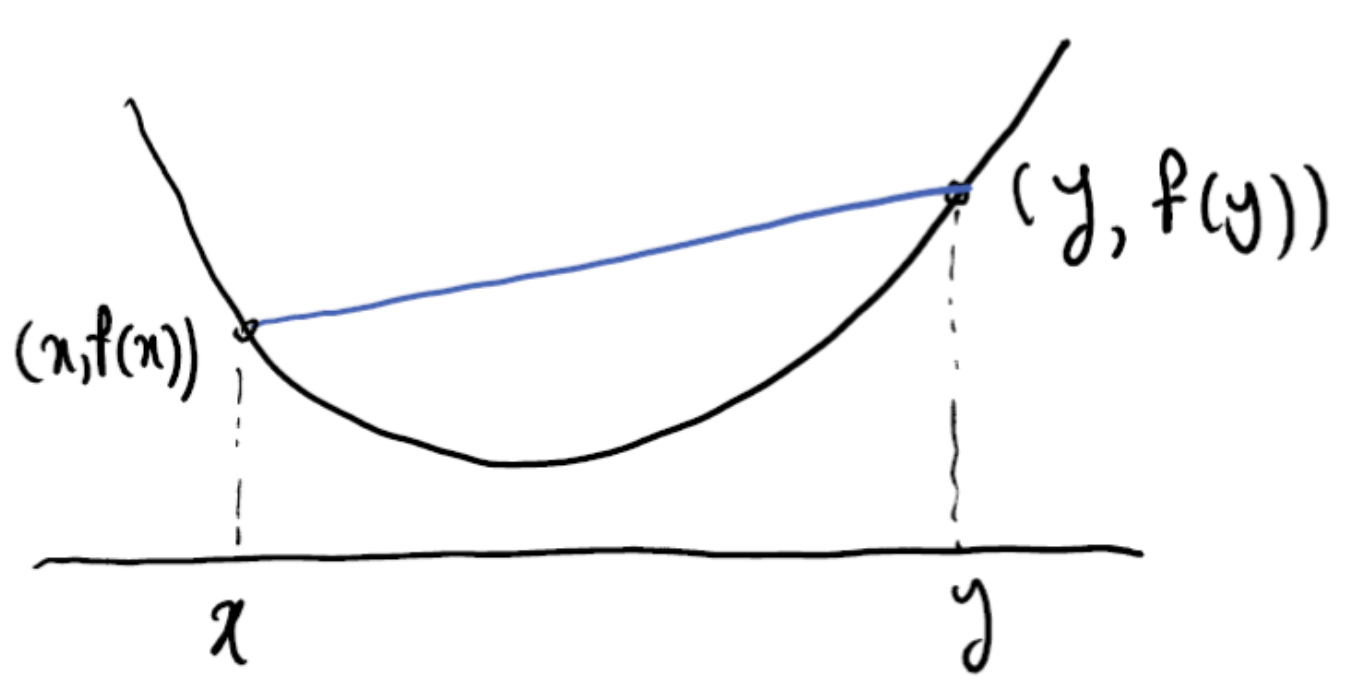
\includegraphics[width=\textwidth]{1.png} 
    \end{figure}

\begin{enumerate}
\item[\textcolor{red}{Solution:}]
\textcolor{red}{
 The approach utilizing exact line search exhibited the quickest convergence to the function's minimum, demonstrating substantial efficacy in optimization. Next was the Armijo line search, which also effectively adjusted step sizes adaptively but at a marginally slower rate. The version without a line search showed the slowest convergence, highlighting the role of line search in enhancing the steepest descent method's convergence speed.
}
\end{enumerate}


  
\item Verify that the Steepest descent method converges to the minimum $x^*$
  for any starting point within the region.


\begin{enumerate}
\item[\textcolor{red}{Solution:}]
\textcolor{red}{
Each approach—without line search, with exact line search, and with Armijo line search—converged towards the function's minimum. This convergence behavior across different starting points confirms the robustness of the steepest descent method in finding the minimum $x^*$ within the specified region.}
\end{enumerate}


    \begin{figure}[H]
    \centering
    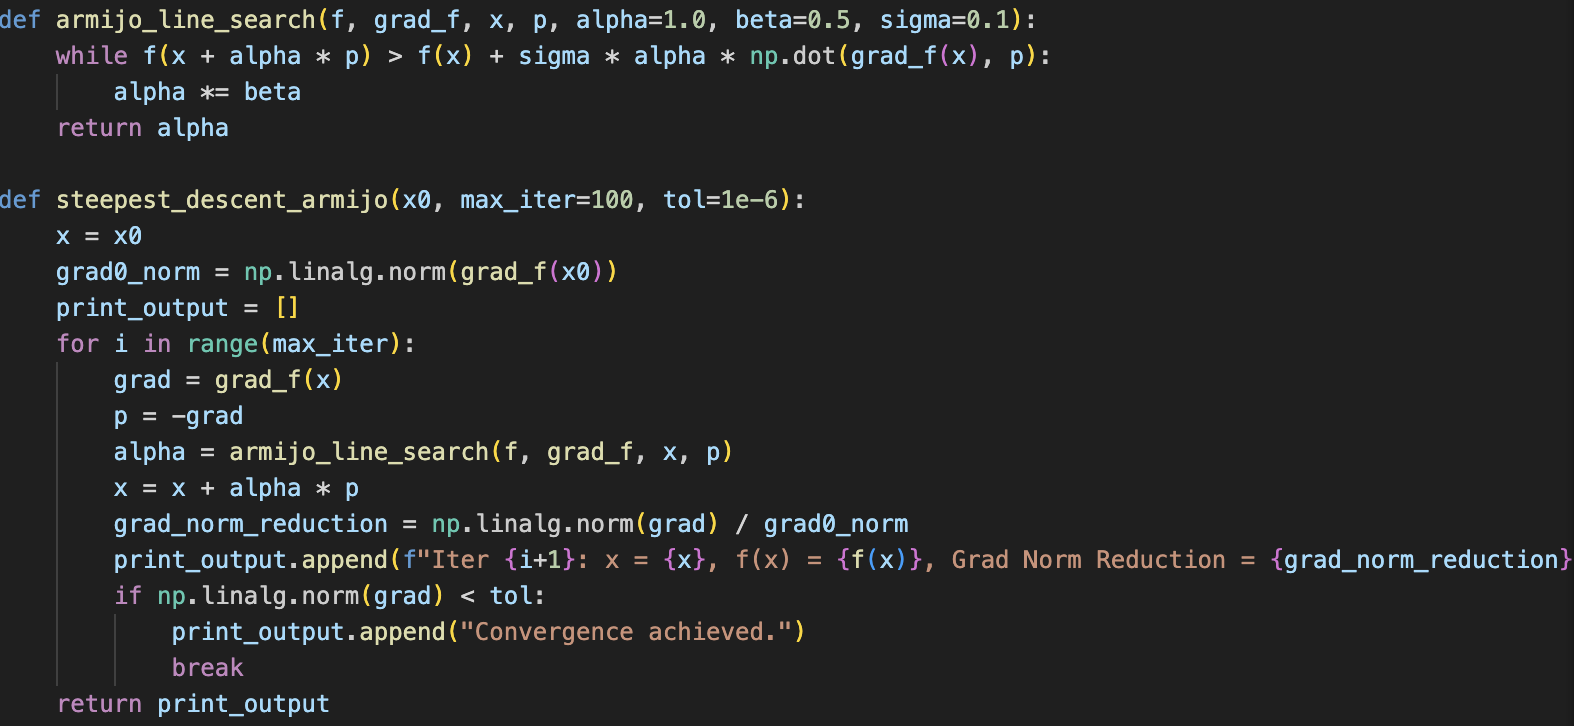
\includegraphics[width=\textwidth]{1a.png} 
    \end{figure}

  
\item What do you observe about the convergence rate in these cases?

\begin{enumerate}
\item[\textcolor{red}{Solution:}]
\textcolor{red}{
The observed convergence rates for the steepest descent method showcased exact line search exhibited the most rapid convergence. The Armijo line search also had efficient convergence by adaptively adjusting step sizes, though at a slightly slower pace compared to the exact line search. Without any line search, the convergence was markedly slower.}
\end{enumerate}






\item ({\bf 5 points}) Use your Matlab implementation of the
  Steepest descent method (with and without line search) to minimize
  \textbf{Rosenbrock's function}, which in two dimensions is given by
  $$
  f(x) = (1 - x_1)^2 + 100(x_2 - x_1^2)^2.
  $$
  Start with initial point $(-1,1)$.




    \begin{figure}[H]
    \centering
    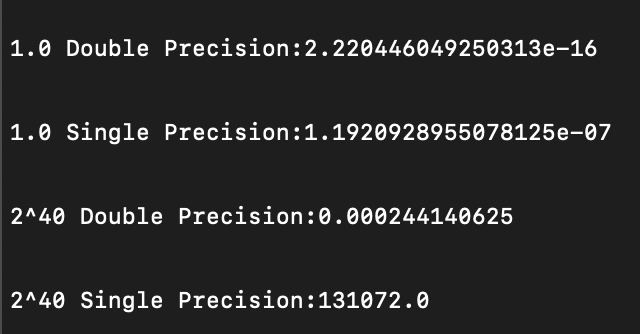
\includegraphics[width=\textwidth]{2.png} 
    \end{figure}

\begin{enumerate}
    \item[\textcolor{red}{Solution:}] 
    \textcolor{red}{
The output indicates that Steepest Descent method without line search is showing very slow convergence towards the minimum of the function. In contrast, the Steepest Descent with Armijo line search shows rapid convergence, achieving the desired tolerance after just two iterations. }
\end{enumerate}





\item ({\bf 5 points}) {\bf \textcolor{red}{Tentative} Project Plan}:

  \begin{enumerate}
  \item If you decide to work with your peers, please submit the names
    of your team members. It's perfectly acceptable to work alone on
    the project as well.





\begin{enumerate}
    \item[\textcolor{red}{Team Members:}] 
    \textcolor{red}{Ronald Nap, Cristian Espinosa
    }
\end{enumerate}



    
  \item (If applicable) Meet with your group initially to start
    discussing a topic. Submit a tentative title.

\begin{enumerate}
    \item[\textcolor{red}{Tentative Title:}] 
    \textcolor{red}{Edge-Aware Image Smoothing via Weighted Least Squares Optimization and Deep Learning}
\end{enumerate}

    
  \item Give a short description of why you are interested on this
    topic.

\begin{enumerate}
    \item[\textcolor{red}{Description:}] 
    \textcolor{red}{My interest in edge promoting stems from enhancing computer vision tasks by preserving edges in image processing.}
\end{enumerate}


    
  \item Include 2-3 references for the topic you chose.

\begin{enumerate}
    \item[\textbf{References:}]
    
    \item \textcolor{red}{``Total Variation Optimization Layers for Computer Vision''} \\
    \href{https://arxiv.org/pdf/2204.03643.pdf}{Paper}, \href{https://github.com/raymondyeh07/tv_layers_for_cv/tree/main}{Code}

    \item \textcolor{red}{``Fast Global Image Smoothing Based on Weighted Least Squares''} \\
    \href{https://ieeexplore.ieee.org/stamp/stamp.jsp?tp=\&arnumber=6942220}{Paper}

    \item \textcolor{red}{``Deep Edge-Aware Filters''} \\
    \href{https://proceedings.mlr.press/v37/xub15.pdf}{Paper}

\end{enumerate}


  
  \item You can meet with me to discuss the project plan and help
    further ideas - come prepared to this meeting with some topics you
    would be interested in. Send an email to set up an appointment.

\begin{enumerate}
\item[\textcolor{red}{Preparation:}]
\textcolor{red}{We intend to prepare a detailed project outline, including a literature review and proposed methodology}
\end{enumerate}
    
  \end{enumerate}

\end{enumerate}
\end{document}